\documentclass[11pt, a4paper, leqno]{article}
\usepackage{a4wide}
\usepackage[T1]{fontenc}
\usepackage[utf8]{inputenc}
\usepackage{float, afterpage, rotating, graphicx}
\usepackage{epstopdf}
\usepackage{longtable, booktabs, tabularx}
\usepackage{fancyvrb, moreverb, relsize}
\usepackage{eurosym, calc}
% \usepackage{chngcntr}
\usepackage{amsmath, amssymb, amsfonts, amsthm, bm}
\usepackage{caption}
\usepackage{mdwlist}
\usepackage{xfrac}
\usepackage{setspace}
\usepackage{xcolor}
\usepackage{subcaption}
\usepackage{minibox}
% \usepackage{pdf14} % Enable for Manuscriptcentral -- can't handle pdf 1.5
% \usepackage{endfloat} % Enable to move tables / figures to the end. Useful for some submissions.


\usepackage[
    natbib=true,
    bibencoding=inputenc,
    bibstyle=authoryear-ibid,
    citestyle=authoryear-comp,
    maxcitenames=3,
    maxbibnames=10,
    useprefix=false,
    sortcites=true,
    backend=biber
]{biblatex}
\AtBeginDocument{\toggletrue{blx@useprefix}}
\AtBeginBibliography{\togglefalse{blx@useprefix}}
\setlength{\bibitemsep}{1.5ex}
\addbibresource{refs.bib}





\usepackage[unicode=true]{hyperref}
\hypersetup{
    colorlinks=true,
    linkcolor=black,
    anchorcolor=black,
    citecolor=black,
    filecolor=black,
    menucolor=black,
    runcolor=black,
    urlcolor=black
}


\widowpenalty=10000
\clubpenalty=10000

\setlength{\parskip}{1ex}
\setlength{\parindent}{0ex}
\setstretch{1.5}


\begin{document}

\title{Skills and Wages\thanks{Poooja Bansal, University of Bonn. Email: \href{mailto:pooja.bansal2610@gmail.com}{\nolinkurl{pooja [dot] bansal2610 [at] gmail [dot] com}}.}}

\author{Poooja Bansal}

\date{
{\bf Preliminary -- please do not quote} 
\\[1ex] 
\today
}

\maketitle


\begin{abstract}
	We provide joint evidence on the relationship between individuals’ cognitive abilities, their personality and earnings for individuals in  Germany using Mincer approach. The paper also estimates the relationships for different categories of occupation defined using the Goldthorpe  classification, 1992. With the data from the German Socio-Economic Panel Study, we employ scores from two short IQ-tests and a set of measures of personality traits which includes items from the Five Factor Personality Inventory. We regress our variables on log hourly wages using different specifications. The results suggest Education and experience are significant factors in the labor market. Our estimates for cognitive abilities indicate no association with wages for any occupations whereas for personality traits, our findings are heterogeneous, varying for different occupations.\\
\\
Keywords: Cognitive skills, Personality traits,SOEP, Occupation, Mincer, Wages \\
\\
Acknowledgement:  We would like to thank Prof.Dr.Thomas Dohmen and Dr.Philipp  Eisenhauer, University of Bonn for providing us with their expertise and guidance during the course of this research.
\end{abstract}
\clearpage

\section{Introduction} % (fold)
\label{sec:introduction}

There has been a growing interest in understanding the effects of non-cognitive skills and personality traits, on labour market outcomes. Many empirical studies have recognized the increasing importance of non-cognitive skills along with the cognitive skills. We try to build on this by studying the effects of both cognitive and non-cognitive skills on individuals’ wage profiles. Since the requirements for these skills vary with different occupations, we investigate the variations  by analyzing how these skills affect the wage profiles of individuals across different occupation levels.\par
The objective of this paper is twofold. We first examine whether cognitive and non-cognitive skills explain difference in hourly wages after controlling for experience and schooling, particularly the relative magnitude of the impact. Secondly we seek to estimate how the skill demands vary across different occupation levels. \par

People typically embody both type of skills: Cognitive skills driving their reasoning and thinking; and non-cognitive skills incorporating their personality traits.
Neisser (1996) defines Cognitive skill as “the ability to understand complex ideas, to adapt effectively to the environment, to learn from experience, to engage in various forms of reasoning, to overcome obstacles by taking thought.” There are numerous studies that have established measurements for cognitive abilities, for instance AFQT scores derived from the Armed Services Vocational Aptitude Battery (ASVAB) , GAT scores test which exists in the Commonwealth nations and IQ performance tests by DIW, Germany. These scores usually approximate cognitive abilities.\par
Most of the literature so far has focused on cognitive abilities only and ignored the importance of non-cognitive skills in labour market analysis due the fallibility of the measures. The skills, popularly known as the personality traits, encompasses many abilities perseverance, patience, reliability, cooperation, emotional stability, self-efficacy, self-esteem and security. Many economists have produced large body of evidence that employers in labor market have recognized the relationship between non-cognitive skills and productivity. This recognition have led to the evolution of measures like  Rosenberg Self esteem scale and Rotter Locus of control, the Big Five Factor Model to study the importance of these in the labor market. \par
The studies so far have discussed the importance of these skills in the labor market. We are contributing to this literature by establishing the relationships between these skills and occupations. But to what extent is occupation useful to understand how education and skills are related with wages. With the rapidly changing trends in the global labor market, employers today want their employees to possess a certain degree of qualification, in terms of skills, education and experience, due to the  non-pecuniary characteristics of different jobs. And in this highly competitive market, employees are keen to develop their qualifications to suit the market needs. Hence we see how these qualifications change in the occupational hierarchy.

This paper continues in the following order: In the next section we will discuss some of the literature which focuses on similar research area that helped us structure our expectations. In the Data section, we describe our data and source. In the Methodology section, we present our econometric framework, followed by the Result section where the first part explains the general relationship of skills for different individuals and then in the second part, we explore the differences in the relationships across various occupational levels. We then provide the robustness checks and finally conclude our analysis.

If you are using this template, please cite this item from the references: \citet{GaudeckerEconProjectTemplates}

\citet{Schelling69} example in the code is taken from \citet{StachurskiSargent13}
fhgfghfchvmnbjjkgu
The decision rule of an agent is the following:
\begin{align*}
    \text{move} & \quad \text{if} \quad n_\text{neighbours} < 4 \\
    \text{stay} & \quad \text{if} \quad n_\text{neighbours} \geq 4
\end{align*}


\begin{figure}
    \caption{Segregation by cycle in the baseline \citet{Schelling69} model as in the \citet{StachurskiSargent13} example}
    
    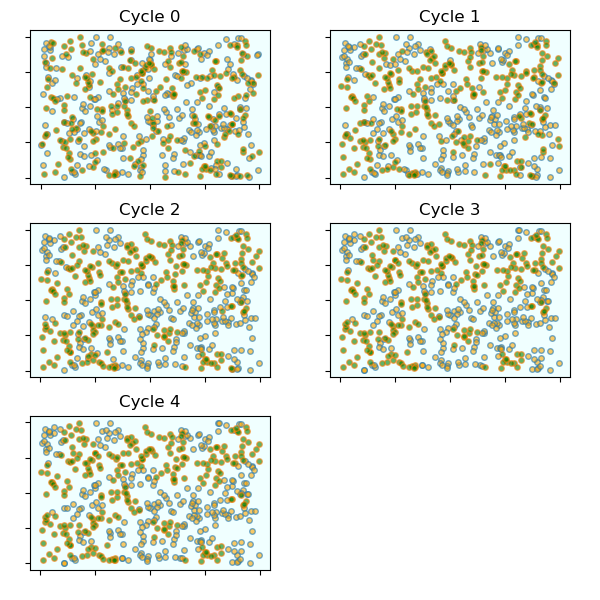
\includegraphics[width=\textwidth]{../../out/figures/schelling_baseline}

\end{figure}


\begin{figure}
    \caption{Segregation by cycle in the baseline \citet{Schelling69} model, limiting the number of potential moves per period to two}
    
    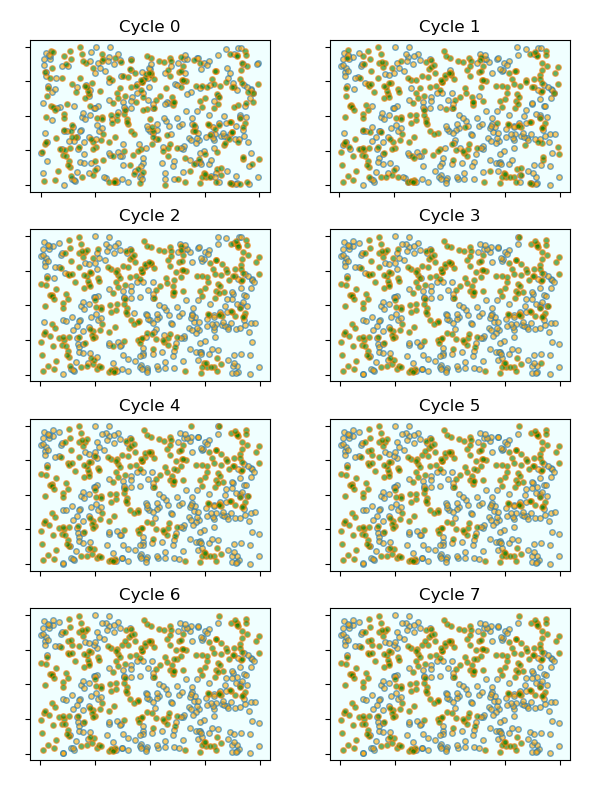
\includegraphics[width=\textwidth]{../../out/figures/schelling_max_moves_2}

\end{figure}

% section introduction (end)




\setstretch{1}
\printbibliography
\setstretch{1.5}




% \appendix

% The chngctr package is needed for the following lines.
% \counterwithin{table}{section}
% \counterwithin{figure}{section}

\end{document}
